\chapter{関連研究}
\label{chap:relatedwork}

2章では自分の研究をより広い研究領域の中に位置付けるため、関連研究の整理を行う。
単純に自分の研究に先行する類似研究を2~3紹介すれば終わりというのではなく、
そもそも取り組んでいる研究領域がどの程度の範囲にまたがるのか、
使っている研究手法や対象データの側面から、どのような研究が行われているのかなど、
学位論文であればページ数が限られないため、かなり広範に述べることが期待される。

とはいえ、いきなり研究領域全体を説明することはものすごく大変なので、
いくつかの軸・観点をつくって、それらを節に分けながら解説する。
可能ならば、冒頭で、全体の軸や観点を整理した図表を使って説明できるとよい。
また、各節の最後には、自分の研究との違いと類似点を簡単にまとめておくことも忘れずにしよう。

例えば、ある修士論文\cite{obata:2018:master}の関連研究の章で示された図をもとに一部改編して示した例を図\ref{fig:relatedwork-overview}に示す。

\begin{figure}[htb]
    \centering
    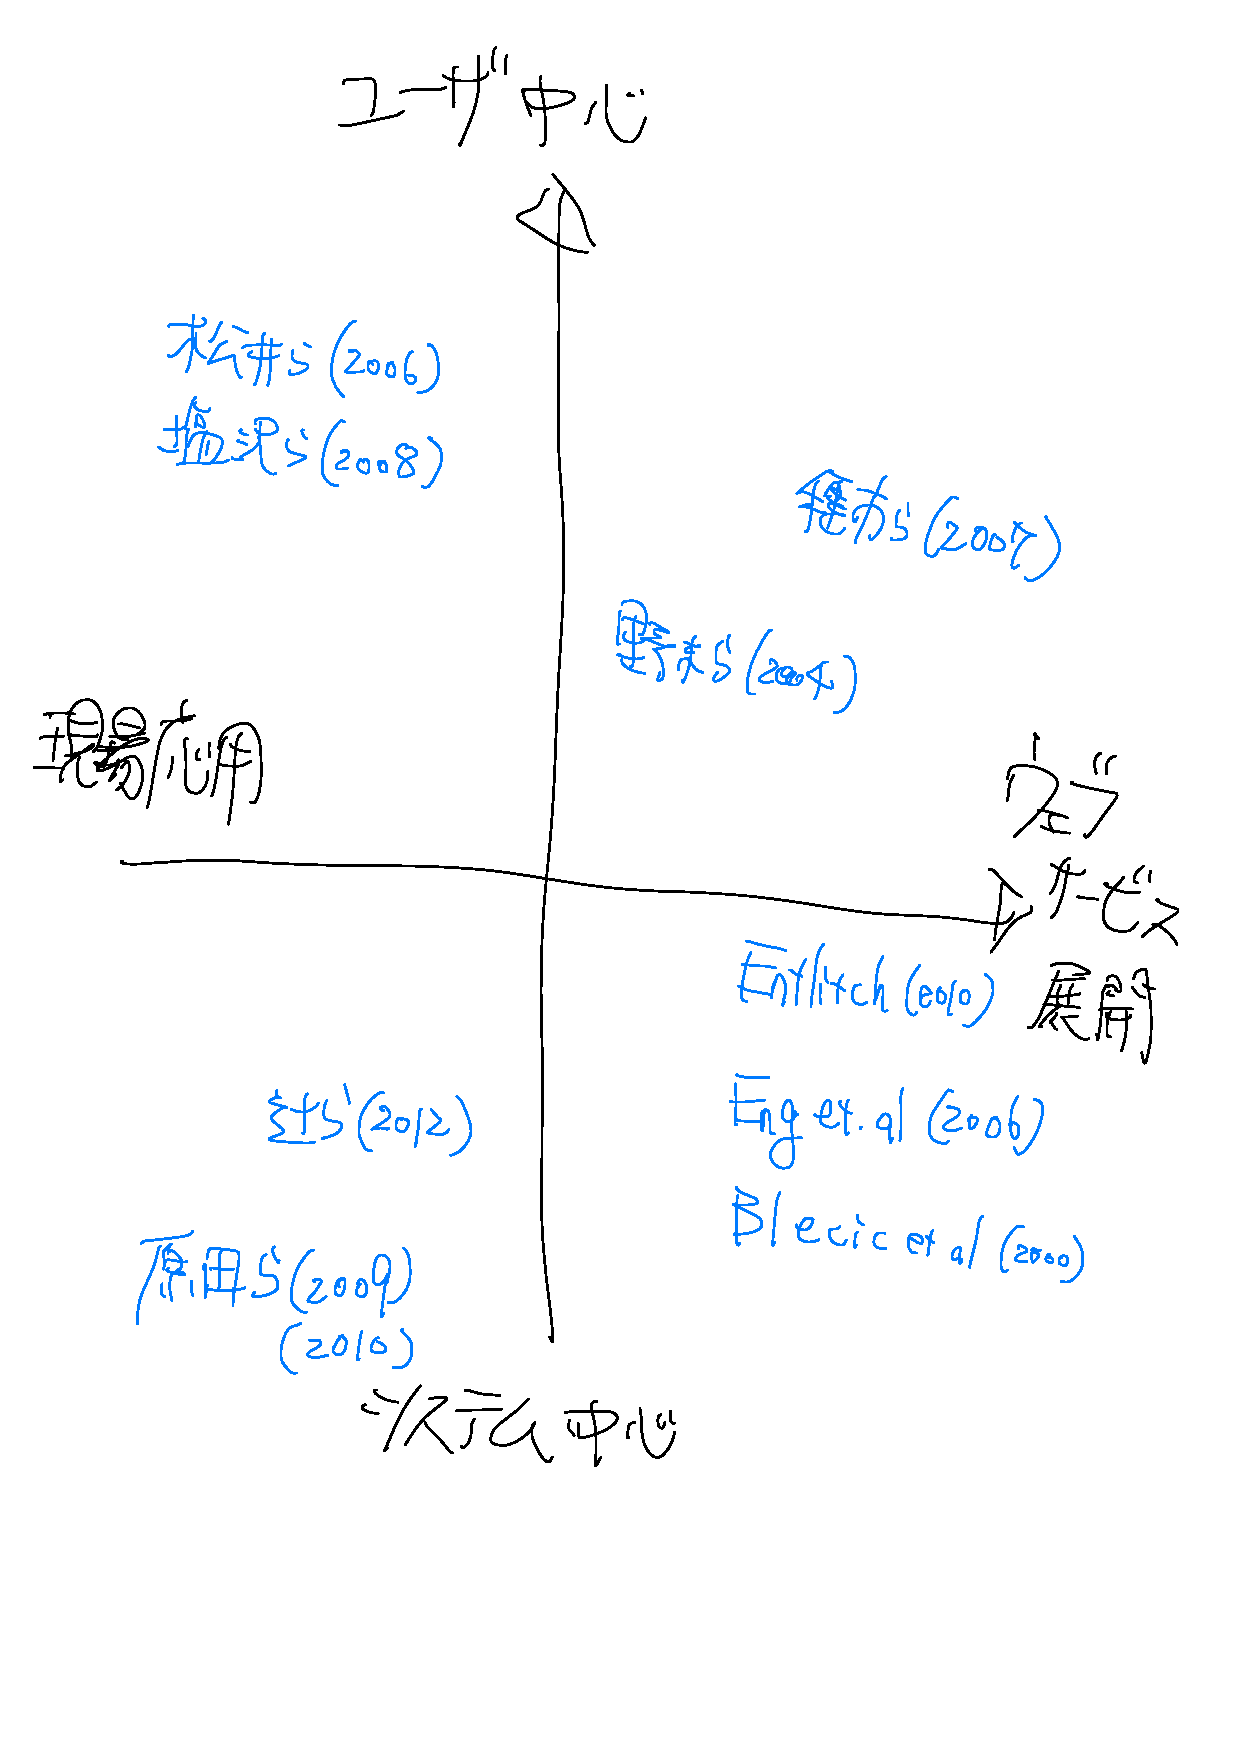
\includegraphics[width=.6\hsize]{figures/relatedwork-overview.pdf}
    \caption{関連研究の概要}
    \label{fig:relatedwork-overview}
\end{figure}
